\section{Instuderingsfrågor}
\label{sec:instudering}
Det är viktigt att ni innan laborationen har en idé om vad ni vill ta
reda på och hur ni vill gå till väga. Därför skall ni senast en studievecka
före ert laborationstillfälle ha besvarat nedanstående frågeställningar
skriftligen.
Variablerna $x_1$, $x_2$ och $x_3$
%$\aleph$, $\beth$ och $\daleth$
är era individuella födelseår
(2-siffrigt), födelsemånad och födelsedag respektive.

\begin{enumerate}
\item Vad händer ifall ni försöker följa reaktionen vid för hög
  temperatur?
\item Vad händer ifall ni försöker följa reaktionen vid för hög
  jonstyrka?
\item Om ni uppmäter en hastighetskonstant vid jonstyrkan $I =
  \SI{0.05}{\mole\per\kg}$, hur skall ni då ändra jonstyrkan så att den
  observerade hastighetskonstanten minskar med 30\%?
\item Vad är jämviktskoncentrationen \ce{FeSCN^{2+}} ifall
  $[\ce{SCN^{-}}]_{tot} = \SI{0.5}{\milli\Molar}$ och 
  $[\ce{Fe^{3+}}]_{tot} = \SI{1.5}{\milli\Molar}$
\item Vad är
  $\frac{\gamma_\ce{FeSCN^{2+}}}{\gamma_\ce{Fe^{3+}}\gamma_\ce{SCN^-}}$
  för $I = x_1~\si{\milli\mole\per\kg}$?
\item Vad är $\frac{[\ce{Fe^{3+}}]}{[\ce{FeOH^{2+}}]}$ vid pH $x_2$?
\item Vad är $[\ce{Fe_2(OH)_2^{4+}}]$ vid pH 2 ifall
  $[\ce{Fe^{3+}}]_{tot} = x_3~\si{\milli\Molar}$?\footnote{
Alternativ 1: försumma bildandet av \ce{FeOH^{2+}}. Alternativ 2: ställ upp ekvationer
för jämvikterna och utnyttja bevarandet av järnatomerna, lös
exempelvis med WolframAlpha.
}
% \item Vad sker med jonstyrkan under reaktionsförloppet i en vattenlösning
%   med stökiometriska mängder järn(III)perklorat och natriumtiocyanat med
%   mycket små halter av åskådarjoner? Hur påverkar det
%   hastighetskonstanten $k_f$?
\item Vad är tänkbara initialkoncentrationer (dvs. vad tror ni kommer att
  fungera bra)? Dessa kan sedan justeras baserat på erhållna data. Se
  \cref{fig:fe} för val av pH.
\item Vad är jonstyrkan vid $t=0$ och $t=\infty$ för era föreslagna
  koncentrationer?
\item Vad är absorbansen vid $t=\infty$ för era föreslagna
  koncentrationer? Vid vilken transmittans tror ni att ni har bäst
  känslighet i er detektor? Vilken absorbans motsvarar det? (Om
  absorbansen är olämplig: ändra då era föreslagna intialkoncentrationer)
\end{enumerate}

\begin{figure}
  \centering
  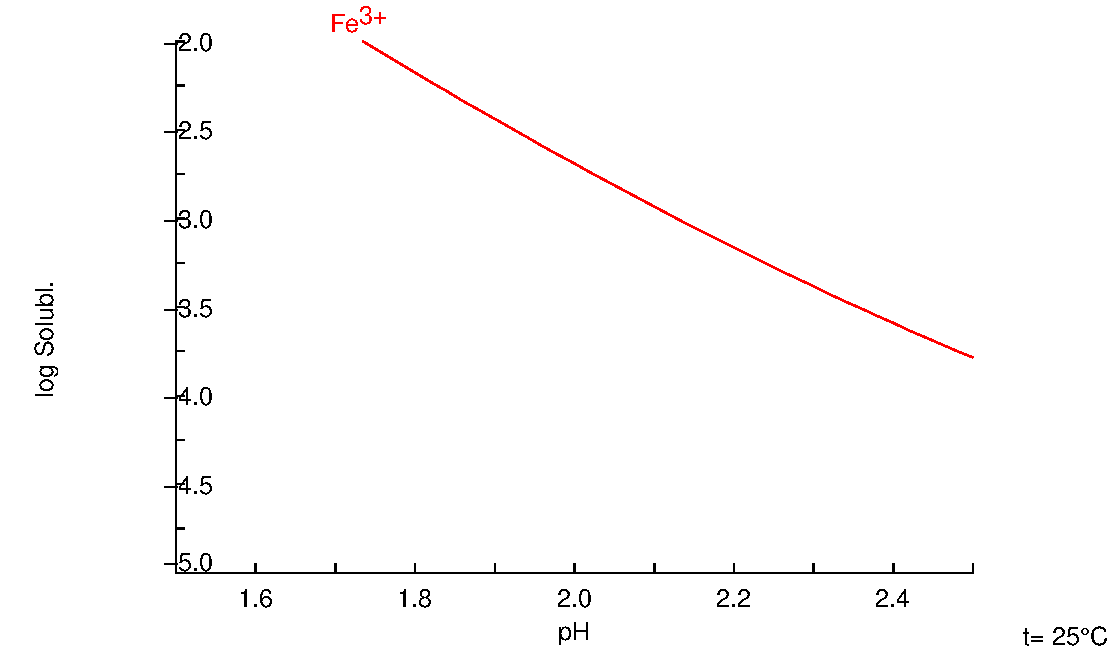
\includegraphics[scale=0.4]{fig/fe.pdf}
  \caption{Löslighetsdiagram för järn(III)}
  \label{fig:fe}
\end{figure}

%%% Local Variables:
%%% mode: latex
%%% TeX-master: "../main"
%%% ispell-local-dictionary: "swedish"
%%% End:
